\section{Laboratory work implementation}

\subsection{Tasks and Points}

\begin{itemize}
	\item Basic Level (nota 5 || 6):
	
	\begin{itemize}
		\item Realizeaza un simplu GUI calculator care suporta functiile de baza: +, -, /, *.
	\end{itemize}
	
	\item Normal Level (nota 7 || 8):
	
	\begin{itemize}
		\item Realizeaza un simplu GUI calculator care suporta urmatoare functii: +, -, /, *, putere, radical, InversareSemn(+/-).
	\end{itemize}
	\item Advanced Level (nota 9 || 10):
	
	\begin{itemize}
		\item Realizeaza un simplu GUI calculator care suporta urmatoare functii: +, -, /, *, putere, radical, InversareSemn(+/-), operatii cu numere zecimale.
	\end{itemize}
	\begin{itemize}
		\item Divizare proiectului in doua module - Interfata grafica(Modul GUI) si Modulul de baza(Core Module).
	\end{itemize}
\end{itemize}

\subsection{Analiza lucrarii de laborator}

Link SSH la repozitoriu: git@github.com:DanielUrsachi/MIDPS.git


Am realizat un calculator in GUI-il QtCreator, folosind instrumentele grafice din si functii matematice. Din punct de vedere vizual am 2 tipuri de obiecte, butoane si textedit-uri, avind o clasa ce le dirijeaza pe toate. Implementarea acestora o putem face prin bara de stinga de instrumente
\begin{center}
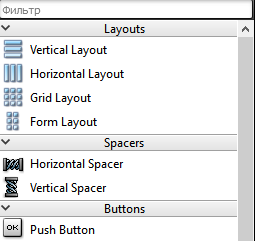
\includegraphics[width=0.6\linewidth]{1stinga}
\end{center}
Actiunile acestor butoane le-am introdus prin click dreapta trecerea la slot
\begin{center}

\includegraphics[width=0.7\linewidth]{11}
\end{center}
Si selectarea optiunii necesare
\begin{center}
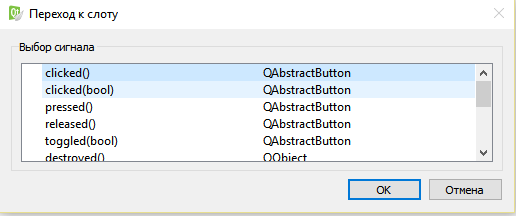
\includegraphics[width=0.7\linewidth]{12}
\end{center}


Am introdus in clasa de baza din clasa.h toate variabilele si functiile ce vor fi folosite.
Din punc de vedere functional, am 4 principii de functii:

	\begin{itemize}
		\item Butoanele cifrele- care introduc valoarea intr-o variabila inmultind cu 10 valoarea precedenta sau in cazul punctului inmultind-o cu 0.1 la puterea numarului elementului de introducere.
	\item Operatiile +,-,*,/,pow care au nevoie de 2 variabile introduse pentru a le calcula, dupa care au nevoie de inca o operatie sau de = pentru afisarea rezultatului
	\item Insusi butonul = si C, care afiseaza valoarea variabilei principale la moment(in cazul C x = 0)
\item 	Operatiile sqrt, ., -/+ care doar schimba valoarea variabilei cu care lucram, ceea ce ne ofara posibilitatea de a actiona prin pasi la ambele argumente dintr-o operatie.
\end{itemize}	
	DIVIZAREA
Toate schimbarile grafice se petrec in calc.cpp de unde doar se apeleaza alte functii pentru calculare aritmetica
Am mai creat un file header (fun.h) pe care l-am introdus in clasa de baza, si in acest file .h am efectuat tot functionalul matematic
\begin{center}
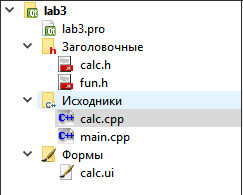
\includegraphics[width=0.7\linewidth]{divizarea}
\end{center}
Forma finala a calculatorului:
\begin{center}
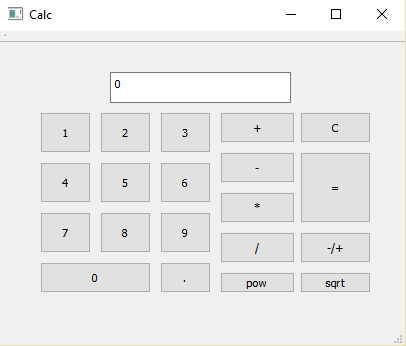
\includegraphics[width=0.7\linewidth]{3calc}
\end{center}

